
\includegraphics[height=1.25cm]{images/pictograms/triangle}

\includegraphics[height=1.25cm]{images/pictograms/bsc}

\includegraphics[height=1.25cm]{images/pictograms/msc}

\includegraphics[height=1.25cm]{images/pictograms/tools}

%%%%%%%%%%%%%%%%%%%%%%%%%%%%%%%%%%%%%%%%%%%%%%%%%%%%%%%%%%%%%%%%%%%%%%%%%%%%%%%%%%%%%%%%%%%%%%%%%%%


\begin{flushright} {\tiny {\color{gray} python\_codes/fieldstone\_131/text.tex}} \end{flushright}

%\lstinputlisting[language=bash,basicstyle=\small]{python_codes/fieldstone_131/keywords}

\begin{center}

\fbox{\textbf{\large \color{teal} P}}
Codes at \url{https://github.com/cedrict/fieldstone/tree/master/python_codes/fieldstone_131}
\end{center}

\par\noindent\rule{\textwidth}{0.4pt}

{\sl This stone was developed in collaboration with M. Blasweiler and J. Wolbers}. 
\index{contributors}{M. Blasweiler}
\index{contributors}{J. Wolbers}

\par\noindent\rule{\textwidth}{0.4pt}
%%%%%%%%%%%%%%%%%%%%%%%%%%%%%%%%%%%%%%%%%%%%%%%%%%%%%%%%%%%%%%%%%%%%%%%%%%%%%%%%%%%%%%%%%%%%%%

In previous stones we have used the {\tt triangle} code \url{https://www.cs.cmu.edu/~quake/triangle.html}.
Although very fast and very stable, this code is written in C and the interface with python 
is therefore not optimal. Typically one would generate the nodes on the convex hull and inner 
material boundaries, write these into a file, have {\tt triangle} read these in, return the 
generated mesh into a file, and read the latter in the FEM python code. 

However, there is a python module which is capable of generating Delaunay triangulations like {\tt triangle}
and we here explore its use. In order to install it:
\begin{verbatim}
pip3 install triangle
\end{verbatim}

\url{https://rufat.be/triangle/delaunay.html}

In the {\python stone.py} you will find five examples illustrating the various 
uses of this library. The code also provides an export to vtu file. 


\begin{center}
\includegraphics[width=8cm]{python_codes/fieldstone_131/example1/example1}
\includegraphics[width=8cm]{python_codes/fieldstone_131/example2/example2}\\
{\captionfont Example 1 (left), example 2 (right)}
\end{center}


\begin{center}
\includegraphics[width=4cm]{python_codes/fieldstone_131/example3/example3}
\includegraphics[width=4cm]{python_codes/fieldstone_131/example4/example4}
\includegraphics[width=4cm]{python_codes/fieldstone_131/example5/example5}
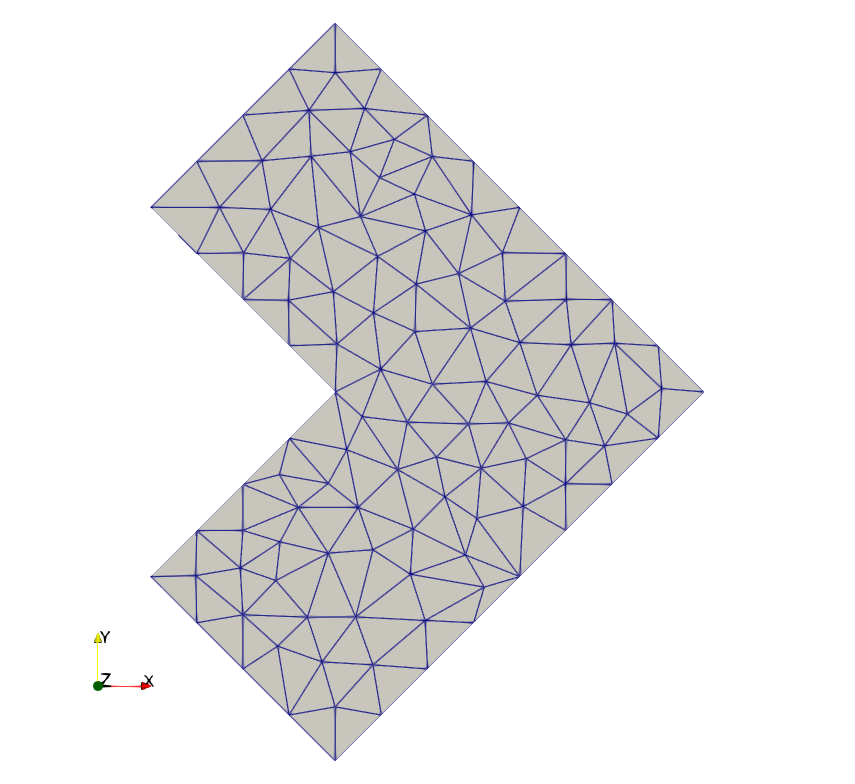
\includegraphics[width=4cm]{python_codes/fieldstone_131/example6/mesh}\\
{\captionfont Examples 3,4,5,6.}
\end{center}

%%%%%%%%%%%%%%%%%%%%%%%%%%%%%%%%%%%%%%%%%%%%%%%%%%
\section*{From linear triangles to quadratic ones}

In the case quadratic triangular elements are to be used a conversion $P_1 \rightarrow P_2$
is provided.

Two methods are implemented. The first one is naive and therefore not efficient at all:
It essentially creates all mid-edges points for all triangles and then looks for those 
that are situated at the same coordinates and remove doubles. 
The second one generates the mid-edge nodes progressively and checks that they do not 
exist yet (by means of a connectivity matrix which registers edges - 
stored as vertices pairs).


The file {\pythonfile stone2.py} contains multiple functions:
\begin{itemize}
\item {\python export\_elements\_to\_vtuP1}
\item {\python export\_elements\_to\_vtuP2}
\item {\python mesh\_P1\_to\_P2\_naive}
\item {\python mesh\_P1\_to\_P2}
\end{itemize}

\begin{center}
\includegraphics[width=8cm]{python_codes/fieldstone_131/P1P2/meshP1}
\includegraphics[width=8cm]{python_codes/fieldstone_131/P1P2/meshP2}\\
{\captionfont $P_1$ mesh (left), $P_2$ mesh (right)}
\end{center}

In the case of a full disc, we vary the number of triangles and find that 
the second algorithm strongly outperforms the first one:
 
\begin{center}
\begin{tabular}{|l|c|c|c|c|}
\hline
                       & 'qa0.003' & 'qa0.002' & 'qa0.001' & 'qa0.0005' \\
nel                    & 1638      & 2408      & 4813 &  9677\\
\hline
P1$\rightarrow$P2 naive& 27.4s      & 53.8s     & 216.6s & 958.5s\\
P1$\rightarrow$P2 smart& 0.071s     & 0.099s    & 0.195s & 0.397s\\
\hline
\end{tabular}
\end{center}




